\section{DevOps}
\label{sec:devops}

O termo DevOps tem sido usado com frequência em diversas esferas do
desenvolvimento de software da atualidade, mas por ser um conceito recente
(2008), muita cunfusão ainda é gerada ao tentar definir e trabalhar com DevOps.
A palavra DevOps vem de duas palavras em ingles, \textit{development} e \textit{operations},
ou seja, desenvolvimento e operações, e de maneira geral é a cultura, movimento
ou conjunto de praticas que incentiva comunicação, colaboração e integração de
desenvolvedores de software e outros profissionais de TI, enquanto automatiza o
processo de entrega de software e mudanças de infraestrutura. ~\cite{loukides2012devops}~\cite{erich2014mapping}

Muitas vezes o termo é confundido com uma nova responsabilidade, ou cargo
dentro de uma empresa que desenvolve software, e por mais que seja possível
ter profissionais que tenham proficiencia nas ferramentas relacionadas a
DevOps, o ideal, como dito anteriormente, é ter uma melhor comunicação,
colaboração e integração entre os times já existentes. As ferramentas
relacionadas à DevOps facilitam esses aspectos, mas o diferencial é a
mudança no processo de desenvolvimento para absorver essas melhorias.

\subsection{Metodologia Ágil e DevOps}

Com a popularização da metodologia de desenvolvimento ágil, que tem, entre outros
objetivos, o de entregar com maior frequência, e melhorar a comunicação entre os
times, é simples fazer a relação de DevOps com esse tipo de desenvolvimento.
DevOps nada mais é do que a implementação de conceitos e mudanças organizacionais
e culturais provenientes do pensamento Ágil. ~\cite{scott2014} DevOps tenta
alcançar entregas mais frequentes ao preparar um ambiente que facilite,
automatize e integre vários dos processos que antes seriam manuais, e mais
sucetíveis a falha e atrasos, o que não é possível sem uma equipe integrada
nesse ambiente. Dessa forma o conceito de entrega contínua e de integração
contínua estão fortemente relacionados à DevOps.

\subsection{Integração Contínua}

Integração contínua é a prática de integrar diversas partes de um software
desenvolvido em diversas frentes, de maneira periódica, ou a cada mudança.
Foi adotado como parte da \textit{extreme programming} (XP) que sugere integrar
partes do software mais de uma vez no dia.

Mesmo não que não se siga desenvolvimento orientado a test (TDD), uma
funcionalidade só está pronta se estiver com seus testes implementados,
levando em consideração metodologias de desenvolvimento ágil. E dessa
forma a integração contínua pode dar retorno com relação aos resultados desses
testes a todo momento que ocorrer uma nova integração do software.

\subsection{Entrega Contínua}

\section{Automação}

\subsection{Infraestrutura como Código}

\subsection{Chef}
\label{sec:chef}

Chef é uma ferramenta de gerenciamento e configuração de infraestrutura criada
pela comunidade Opscode em 2008 oficialmente lançada em 2009. Seu propósito é
auxiliar na transformação de uma complexa infraestrutura em código com nível
de abstração compreensiveis para os desenvolvedores de software. Sendo assim,
a gerência de configuração gira em torno da codificação simplificada e amigável
ou invés de comandos manuais de instalação e configuração de aplicações
\cite{sharma:2015}.

\begin{figure}[h]
  \label{fig:arch_chef}
  \centering
  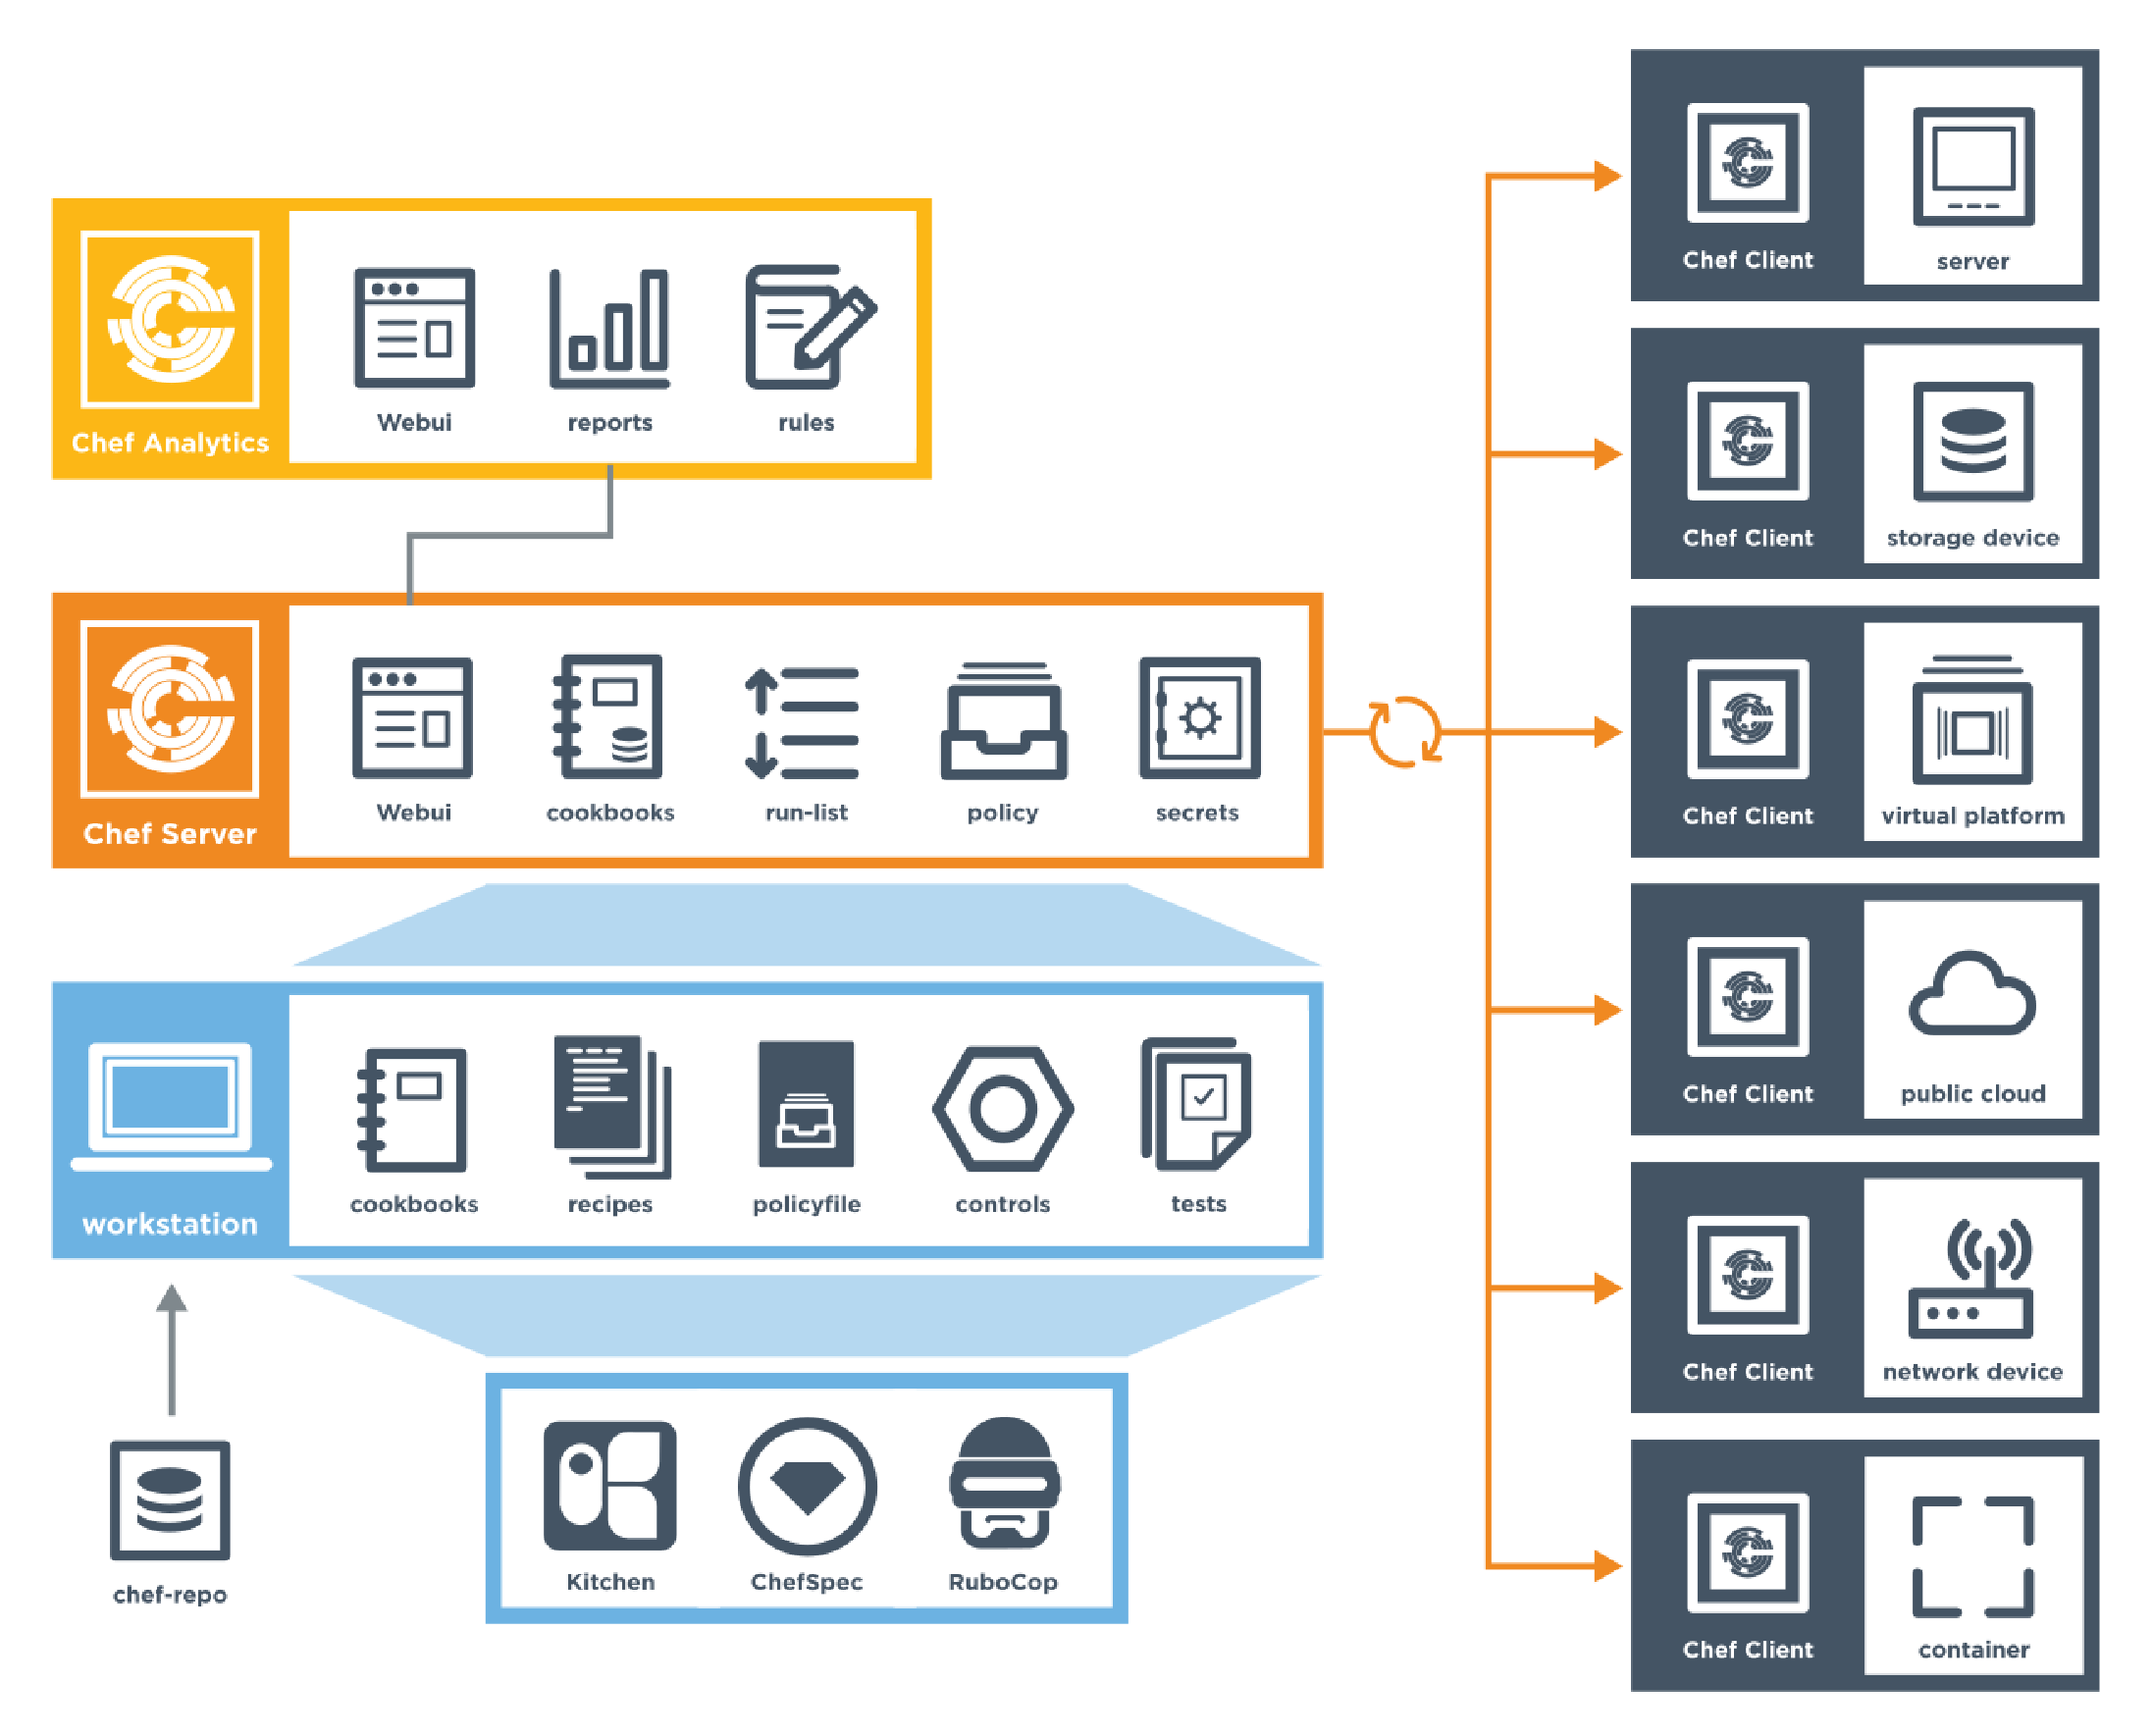
\includegraphics[width=\textwidth]{figuras/arch_chef.eps}
  \caption{Chef - Arquitetura de Componentes}
\end{figure}

